\documentclass{beamer}
\usepackage{amsmath,amsfonts,amsthm,amstext,amssymb, xcolor, tikz, pgf}

% ----------------------------------------------------------
% Theme Setup

% Use Metropolis Theme
\usetheme[numbering=fraction]{metropolis}
\setbeamertemplate{blocks}[rounded][shadow=false]
\makeatletter
\setlength{\metropolis@titleseparator@linewidth}{1pt}
\makeatother



% Define Colors
\definecolor{chargerblue}{HTML}{002764}
\definecolor{chargerred}{HTML}{e02034}
\definecolor{bggray}{HTML}{d0d3d4}

% Set Colors
\setbeamercolor{title}{fg=chargerblue}
\setbeamercolor{background canvas}{bg=white}
\setbeamercolor{title separator}{fg=chargerred}
\setbeamercolor{structure}{fg=chargerblue}
\setbeamercolor{frametitle}{fg=white, bg=chargerblue}
\setbeamercolor*{normal text}{fg=chargerblue}
\setbeamercolor*{block body}{bg=bggray}
\setbeamercolor*{block title}{bg=chargerblue, fg=white}
% ----------------------------------------------------------

% ----------------------------------------------------------
% Custom Definitions, Commands, Environments, etc.

% Sets of numbers
\def\R{\mathbb{R}} % The reals
\def\N{\mathbb{N}} % The naturals
\def\Z{\mathbb{Z}} % The integers
\def\Q{\mathbb{Q}} % The rationals

% Blank space
\newcommand{\blank}[1]{\underline{\hspace{#1}}} % Blank space

% Fitted inclusion symbols
\newcommand{\fp}[1]{\left({#1}\right)} % Fitted parentheses around content
\newcommand{\fb}[1]{\left[{#1}\right]} % Fitted brackets
\newcommand{\set}[1]{\left\{{#1}\right\}} % Fitted braces (useful for sets)
\newcommand{\av}[1]{\left|{#1}\right|} % Fitted absolute value bars

% Coordinate Plane (Four-Quadrant)
\def\coordplane {
	\begin{tikzpicture}
		\draw[step=0.25cm,black,very thin,opacity=0.25] (-2.5cm, -2.5cm) grid (2.5cm, 2.5cm);
		\draw[<->,thick,black] (-2.5cm, 0) -- (2.5cm, 0) node[anchor=north west,pos=0.94,font=\scriptsize]{$x$};
		\draw[<->,thick,black] (0,-2.5cm) -- (0, 2.5cm) node[anchor=south east,font=\scriptsize,pos=0.94]{$y$};
	\end{tikzpicture}
}

% Coordinate Plane (One-Quadrant)
\def\onequad {
	\begin{tikzpicture}
		\draw[step=0.25cm, black, very thin, opacity=0.25] (0,0) grid (7.5cm,5cm);
		\draw[->, thick, black] (0,0) -- (7.5cm, 0) node[anchor=north west,font=\scriptsize,pos=0.94]{$x$};
		\draw[->, black, thick] (0,0) -- (0,5cm) node[anchor=south east,font=\scriptsize,pos=0.94]{$y$};
	\end{tikzpicture}
}
% ----------------------------------------------------------


% ----------------------------------------------------------
% Presentation Information 
\title[2.6 and 2.7]{Operations with Functions; Inverse Functions}
\subtitle{Sections 2.6 and 2.7}
\author{Jacob Ayers}
\institute{Lesson \#10}
\date{MAT 130}
% ----------------------------------------------------------

\begin{document}

% Slide 1 (Title Slide)
\begin{frame}
\titlepage
\end{frame}

% Slide 2 (Objectives)
\begin{frame}[t]{Objectives}
\begin{itemize}
	\item Add, subtract, multiply, and divide functions
	\item Compose Functions
	\item Verify inverse functions graphically and algebraically
	\item Use the Horizontal Line Test to determine whether a function is one-to-one
	\item Find inverse functions algebraically
\end{itemize}

\end{frame}\begin{frame}[t]{Operations with Functions}
\begin{block}{Sum, Difference, Product, Quotient of Functions}
Let $f$ and $g$ be functions with overlapping domains. Then for all $x$ common to both domains, the sum, difference, product and quotient of $f$ and $g$ are defined as follows:

Sum: $(f + g)(x) = f(x) + g(x)$ \vspace{12pt}

Difference: $(f - g)(x) = f(x) - g(x)$ \vspace{12pt}

Product: $(fg)(x) = f(x) \cdot g(x)$ \vspace{12pt}

Quotient: $\fp{\dfrac{f}{g}}(x) = \dfrac{f(x)}{g(x)} \; \text{ provided } g(x) \neq 0$
\end{block}
\end{frame}

\begin{frame}[t]{Operations with Functions}
Suppose that $f(x) = x^2 + 6x + 5$ and $g(x) = x^2 - 4x - 21$. Find $(f + g)(x)$ and $(g - f)(x)$.
\end{frame}

\begin{frame}[t]{Operations with Functions}
Suppose that $f(x) = x^2 - 1$ and $g(x) = x - 1$. Find $(fg)(x)$ and $\fp{\dfrac{f}{g}}(x)$.
\end{frame}

\begin{frame}[t]{Composing Functions}
\begin{block}{Definition}
The \textit{composition} of the function $f$ with the function $g$ is \vspace{-8pt} $$(f\circ g)(x) = f\fb{g(x)}$$ \vspace{-8pt}
\end{block}

\pause

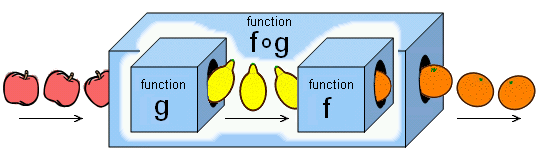
\includegraphics[width=4in]{CompIllustration.png}
\end{frame}

\begin{frame}[t]{Composing Functions}
Suppose that $f(x) = 2x + 5$ and $g(x) = 4x^2 + 1$. Find $f\circ g$ and $g\circ f$
\end{frame}

\begin{frame}[t]{Composing Functions}
Suppose that $f(x) = \sqrt{x-2}$ and $g(x) = x^2 + 2$. Find $f\circ g$ and $g\circ f$.
\end{frame}

\begin{frame}[t]{An Application}
The number $N$ of bacteria in a refrigerated food is given by $$N(T) = 8T^2 - 14T + 200, 2\leq T\leq 12$$ where $T$ is the temperature of the food in degrees Celsius. When the food is removed from refrigeration, the temperature of the food is given by $$T(t) = 2t+2, 0\leq t \leq 5$$ where $t$ is the time in hours. \begin{enumerate}[(a)]
\item Find and interpret $N\circ T$
\item Find the time when the bacteria count reaches 1000.
\end{enumerate}
\end{frame}

\begin{frame}[t]{Inverse Functions}
We saw earlier that $f\circ g$ and $g\circ f$ might come out to the same answer, and they might not.

\pause

It turns out that functions for which $f\circ g = x$ and $g\circ f = x$ are special - they are called \textit{inverses} of one another. \vspace{12pt}

\pause

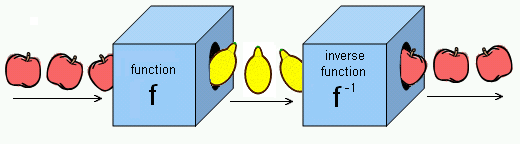
\includegraphics[width=4in]{InvIllustration.png}
\end{frame}

\begin{frame}[t]{Inverse Functions}
\begin{block}{Definition}
Let $f$ and $g$ be functions such that $f\circ g = g\circ f = x$. \vspace{12pt}

Then $g$ is the \textit{inverse} function of $f$ (and vice versa). We denote $g = f^{-1}$ (read ``$f$-inverse") \vspace{12pt}

So $f\fb{f^{-1}(x)} = f^{-1}\fb{f(x)} = x$. \vspace{12pt}

Note that in order for two functions to be inverses, the domain of $f$ must be the same as the range of $f^{-1}$, and the range of $f$ must be the same as the domain of $f^{-1}$.
\end{block}

\pause

It is important to remember that $f^{-1}$ represents the inverse of $f$, not its reciprocal.
\end{frame}

\begin{frame}[t]{Verifying Inverse Functions Algebraically}
Verify that $f(x) = \dfrac{x-4}{7}$ and $g(x) = 7x + 4$ are inverses of each other.

\end{frame}

\begin{frame}[t]{Verifying Inverse Functions Graphically}
The graphs of $f$ and $f^{-1}$ are related in the following way:
\pause

If $(a,b)$ is on the graph of $f$, then $(b,a)$ is on the graph of $f^{-1}$.

Example: Verify that $f(x) = x^2 + 1 (x\geq 0)$ and $g(x) = \sqrt{x-1}$ are inverses.
\end{frame}

\begin{frame}[t]{One-To-One Functions and HLT}
\begin{block}{Definition}
A function is \textit{one-to-one} if and only if each value of the dependent variable ($y$) maps to exactly one value of the independent variable ($x$). A function $f$ has an inverse if and only if it is one-to-one.
\end{block}

\pause

\begin{block}{Horizontal Line Test}
A function $f$ is one-to-one and has an inverse if and only if no horizontal line intersects its graph more than once.
\end{block}

\pause

Example: Determine whether each function has an inverse: (a) $f(x) = x^2$ and (b) $f(x) = \dfrac12\fp{3-x}$. \pause \\ (a) NO \hspace{1in} (b) YES
\end{frame}

\begin{frame}[t]{Finding Inverse Functions Algebraically}
\begin{block}{Finding an Inverse Function}
\begin{enumerate}[1)]
\item Use HLT to determine if $f$ has an inverse.
\item In the equation for $f(x)$, replace $f(x)$ with $y$.
\item Interchange the roles of $x$ and $y$; solve for $y$.
\item Replace $y$ with $f^{-1}$ in the new equation.
\item Verify that $f\circ f^{-1} = f^{-1}\circ f = x$.
\end{enumerate}
\end{block}
\end{frame}

\begin{frame}[t]{Finding Inverse Functions Algebraically}
Find the inverse function of $f(x) = \dfrac{5-3x}{x+2}$.

\pause \vfill

Find the inverse function of $f(x) = \sqrt[3]{10 + x}$.
\end{frame}

\begin{frame}[t]{Next Steps}
\begin{itemize}
\item Complete Assignment \#5
\item Prepare for and take Exam 1
\begin{itemize}
	\item Study guide posted on Moodle in Week 6 (NOT for a grade, but highly recommended)
	\item Exam 1 - Wednesday of Week 7
\end{itemize}
\item Begin Module 7
\begin{itemize}
	\item Read 3-1 and 3-2
	\item Watch Video Lesson \#11
\end{itemize}
\end{itemize}

\vfill

Thanks for watching!
\end{frame}

\end{document}